\chapter{Interruptores automáticos de baja tensión}
\section{Intensidad Nominal}
Es la intensidad de diseño que puede soportar un dispositivo de forma permanente en unas condiciones determinadas sin sufrir ninguna alteración o daño.
\newline
Se define para unas condiciones concretas:
\begin{itemize}
	\item Frecuencia: cambia el comportamiento de la onda
	\item Temperatura ambiente: normalmente 30$^\circ$C, afecta a los esfuerzos térmicos
	\item Condiciones de instalación: afecta a los esfuerzos térmicos y mecánicos
	\item Altitud sobre el nivel del mar: si el aire es menos denso disipa peor
	\item Humedad o contaminación
\end{itemize}
\section{Sobreintensidad de sobrecarga}
Es la intensidad superior a la nominal que puede ser soportada dentro de unos límites de magnitud y tiempo. Se puede deber a una mala previsión de las cargas, transitorios, faltas con alta impedancia,...
\textbf{Origina esfuerzos térmicos}.
\begin{equation}
	Q=\int_{0}^{t} RI^2dt=RI^2t
\end{equation}
\section{Intensidad de cortocircuito}
Es el aumento rápido y elevado de la intensidad, debido a la conexión accidental entre fases o entre éstas y tierra. Depende de las impedancias de los distintos elementos entre el generador y la falta. \textbf{Origina esfuerzos térmicos y mecánicos}.
\section{Funciones de un interruptor automático en baja tensión}
Los interruptores automáticos deben ser capaces de realizar las siguientes funciones:
\begin{itemize}
	\item Cerrar el circuito (\textbf{Establecer}): como es un elemento protector debe ser de capaz de cerrar con la corriente de cortocircuito, pues si no es posible que no funcione adecuadamente
	\item Conducir la corriente (\textbf{Soportar}): debe aguantar los calentamientos y esfuerzos electrodinámicos de la corriente asignada o nominal
	\item Apertura del circuito (\textbf{Interrumpir}): debe poder abrirse mediante alguno de los siguientes mecanismos:
	\begin{itemize}
		\item Acción manual
		\item Relé de sobreintensidad
		\item Relé auxiliar
	\end{itemize}
	\item Seccionamiento (\textbf{Proteger}): debe mantener un nivel de aislamiento suficiente para que no pueda crearse un arco entre partes conductoras (UNE EN 60947-2)
\end{itemize}
\section{Apertura de un circuito}
Una protección puede querer accionarse en vacío (sin intensidad circulando), en funcionamiento normal o en falta (sobrecarga o cortocircuito). 
\newline

El circuito equivalente monofásico de un cortocircuito es el siguiente:
\begin{figure}[H]
	\centering
	\begin{adjustbox}{width=1\textwidth}
		\begin{circuitikz}
			\tikzstyle{every node}=[font=\normalsize]
			\draw (3.5,12.25) to[sinusoidal voltage source, sources/symbol/rotate=auto] (3.5,9.25);
			\draw (4,12.25) to[R] (6.5,12.25);
			\draw (6.5,12.25) to[L ] (9,12.25);
			\draw (4,12.25) to[short] (3.5,12.25);
			\draw (12.25,12.25) to[european resistor] (12.25,9.25);
			\draw (3.5,9.25) to[short] (12.25,9.25);
			\draw (10.25,12.25) to[short] (12.25,12.25);
			\draw [short] (8.75,12.5) -- (9.25,12);
			\draw [short] (8.75,12) -- (9.25,12.5);
			\draw [short] (10.25,12.25) -- (9.5,11.75);
			\draw [->, >=Stealth] (10,11) -- (10.75,12.25);
			\draw [short] (10,11) -- (10.5,11);
			\draw [short] (10.5,11) -- (9.5,9.25);
			\draw [ color={rgb,255:red,251; green,0; blue,255}, ->, >=Stealth] (7.75,9.5) -- (5.5,9.5);
			\draw [ color={rgb,255:red,251; green,0; blue,255}, ->, >=Stealth] (9.5,11.5) -- (9,12);
			\node [font=\normalsize, color={rgb,255:red,251; green,0; blue,255}] at (9,11.5) {$U_a$};
			\node [font=\normalsize, color={rgb,255:red,251; green,0; blue,255}] at (6.5,9.75) {$i_{cc}$};
			\node [font=\normalsize, color={rgb,255:red,1; green,1; blue,1}] at (7.75,12.75) {$L$};
			\node [font=\normalsize, color={rgb,255:red,1; green,1; blue,1}] at (12.75,10.75) {$Z$};
			\node [font=\normalsize, color={rgb,255:red,1; green,1; blue,1}] at (5.25,12.75) {$R$};
			\node [font=\normalsize, color={rgb,255:red,1; green,1; blue,1}] at (2.75,10.75) {$e$};
		\end{circuitikz}
			\end{adjustbox}
	\label{fig:my_label}
\end{figure}

\begin{equation}
	e=Ri_{cc}+L\dfrac{di_{cc}}{dt}+U_a \rightarrow \text{Si el circuito es muy inductivo} \rightarrow L\dfrac{di_{cc}}{dt}=e-U_a 
\end{equation}

La corriente de cortocircuito es máxima si:
\begin{equation}
	e=U_a \rightarrow I_{cc} \text{ es máxima}
\end{equation}

Donde la energía liberada en el arco se define como:
\begin{equation}
	E_a=\int_{0}^{t_a}U_a i_{cc}\,dt
\end{equation}

Donde $U_a$ es la tensión de arco, $i_{cc}$ la intensidad de cortocircuito y $t_a$ la duración del arco.
\newline

\begin{figure}[H]
	\centering
	\begin{minipage}{0.55\textwidth}
		\begin{adjustbox}{width=1\textwidth}
		\begin{circuitikz}
			\tikzstyle{every node}=[font=\normalsize]
			\draw [ color={rgb,255:red,187; green,0; blue,255}, dashed] (3.75,9) -- (3.75,11.75);
			\draw [ color={rgb,255:red,187; green,0; blue,255}, dashed] (10.75,9.25) -- (10.75,11.25);
			\draw [ color={rgb,255:red,0; green,238; blue,255}, dashed] (3.75,11.75) -- (3,11.75);
			\draw [ color={rgb,255:red,0; green,238; blue,255}, dashed] (10.75,11.25) -- (3.75,11.25);
			\draw [ fill={rgb,255:red,171; green,171; blue,171} , line width=0.3pt ] (0,14) rectangle (3.25,13.25);
			\draw [ fill={rgb,255:red,171; green,171; blue,171} , line width=0.3pt ] (11.25,14) rectangle (15.5,13.25);
			\draw [ color={rgb,255:red,255; green,255; blue,255}, line width=0.5pt, short] (15.5,14) -- (15.5,13.25);
			\draw [ color={rgb,255:red,255; green,255; blue,255}, line width=0.5pt, short] (0,14) -- (0,13.25);
			\draw [dashed] (3.25,13.25) -- (3.25,8);
			\draw [dashed] (11.25,13.25) -- (11.25,8);
			\draw [short] (2.75,6.25) -- (11.75,6.25);
			\node [font=\normalsize] at (3.25,6) {0};
			\node [font=\normalsize] at (11.25,6) {L};
			\node [font=\normalsize] at (3.25,14.25) {Ánodo};
			\node [font=\normalsize] at (11.25,14.25) {Cátodo};
			\draw [short] (2.75,10.25) -- (11.75,10.25);
			\draw [short] (3.25,6.25) -- (3.25,9.25);
			\draw [short] (3.25,10.25) -- (3.25,12.75);
			\draw [short] (3.25,12.75) -- (3.75,11.75);
			\draw [short] (3.75,11.75) -- (10.75,11.25);
			\draw [short] (10.75,11.25) -- (11.25,10.25);
			\draw [ color={rgb,255:red,0; green,238; blue,255}, dashed] (3.75,11.25) -- (3,11.25);
			\node [font=\normalsize] at (2.75,12.25) {$U_A$};
			\node [font=\normalsize] at (2.75,10.75) {$U_C$};
			\node [font=\normalsize] at (2.75,11.5) {$U_L$};
			\draw [<->, >=Stealth] (2.25,12.75) -- (2.25,10.25);
			\node [font=\normalsize] at (1.75,11.5) {$U_a$};
			\draw [short] (3,9.25) -- (3.25,9.25);
			\draw [short] (3,8.5) -- (3.25,8.5);
			\draw [short] (3,7.75) -- (3.25,7.75);
			\draw [short] (3,7) -- (3.25,7);
			\node [font=\normalsize] at (2.5,9.25) {8000};
			\node [font=\normalsize] at (2.5,8.5) {6000};
			\node [font=\normalsize] at (2.5,7.75) {4000};
			\node [font=\normalsize] at (2.5,7) {2000};
			\draw [short] (3.25,6.25) -- (3.25,8.25);
			\draw [short] (3.25,7.75) .. controls (3.5,9.25) and (4,9.25) .. (4.25,8);
			\draw [short] (10.25,8) .. controls (10.75,9.75) and (10.75,9.75) .. (11.25,8);
			\draw [short] (11.25,8) -- (11.25,6.25);
			\draw [short] (4.25,8) .. controls (4.5,7) and (6.5,7.5) .. (7.5,7.5);
			\draw [short] (7.5,7.5) .. controls (9,7.5) and (10,7.5) .. (10.25,8);
			\node [font=\normalsize] at (2.5,9.75) {$\theta \left(^\circ C \right)$};
		\end{circuitikz}
	\end{adjustbox}
	\end{minipage}
	\begin{minipage}{0.4\textwidth}
		Por tanto, para que se pueda abrir el circuito eléctrico se debe extinguir el arco eléctrico.
		\begin{equation}
			U_a=U_{AC}+L\cdot U_L
		\end{equation}
		
		Donde, $U_{AC}$ caída de tensión anódica y catódica $\approx 40 V$, $L$ longitud de arco y $U_L$ la caída de tensión por unidad de longitud $\approx 50-100 V/cm$.
	\end{minipage}
\end{figure}

Estos valores se ven afectados por distintos factores como:
\begin{itemize}
	\item Material de los contactos
	\item Medio: se puede mejorar interponiendo de materiales de alta rigidez dieléctrica
	\item Presión se puede mejorar aumentando la presión del medio
	\item Temperatura: se puede mejorar refrigerando el arco
	\item Longitud del arco: se puede mejorar aumentando la longitud del arco
\end{itemize}

Por tanto, para que que se extinga el arco completamente la tensión para el reencendido debe ser mayor a la tensión transitoria de restablecimiento.
\begin{figure}[H]
	\centering
	\begin{minipage}{0.55\textwidth}
		\begin{adjustbox}{width=1\textwidth}
		\begin{circuitikz}
			\tikzstyle{every node}=[font=\normalsize]
			\begin{scope}[rotate around={-1.75:(2,9)}]
				\draw[domain=2:8,samples=100, color={rgb,255:red,0; green,8; blue,255}, ] plot (\x,{4*sin(0.5*\x r -2/0.92*0.5r) +9.35});
			\end{scope}
			\draw [->, >=Stealth] (2,8.25) -- (2,14.25);
			\draw [->, >=Stealth] (1.25,9) -- (10,9);
			\begin{scope}[rotate around={-1.75:(1.75,11)}]
				\draw[domain=2:8,samples=100, color={rgb,255:red,255; green,0; blue,0}, ] plot (\x,{4.2*sin(0.4*\x r -0 r ) +9.35});
			\end{scope}
			\node [font=\normalsize, color={rgb,255:red,255; green,0; blue,0}] at (3,13.4) {$e$};
			\draw[domain=2:5.85,samples=100, color={rgb,255:red,166; green,0; blue,255}, ] plot (\x,{2*sin(0.9*\x r -2/0.92*0.9 r ) +9.35});
			\node [font=\normalsize, color={rgb,255:red,0; green,8; blue,255}] at (7.75,13) {$i_{prevista}$};
			\node [font=\normalsize, color={rgb,255:red,166; green,0; blue,255}] at (5,11.3) {$i_{limitada}$};
			\draw [ color={rgb,255:red,68; green,255; blue,0}, short] (2,9) -- (2.5,9);
			\draw [ color={rgb,255:red,68; green,255; blue,0}, short] (2.5,9) -- (3.75,13);
			\draw [ color={rgb,255:red,68; green,255; blue,0}, short] (3.75,13) -- (4,14);
			\draw [ color={rgb,255:red,68; green,255; blue,0}, short] (5.85,9) -- (5.85,14);
			\draw [ color={rgb,255:red,68; green,255; blue,0}, short] (4,14) -- (5.85,14);
			\draw [dashed] (3.87,13.35) -- (3.87,9);
			\node [font=\normalsize] at (2.5,8.75) {$t_1$};
			\node [font=\normalsize] at (3.87,8.75) {$t_2$};
			\node [font=\normalsize] at (5.85,8.75) {$t_3$};
			\draw [dashed] (2.5,9) -- (2.5,10);
			\draw [dashed] (2.5,10) -- (2,10);
			\node [font=\normalsize] at (1.75,10) {S};
			\node [font=\normalsize] at (1.75,8.75) {O};
			\node [font=\normalsize, color={rgb,255:red,68; green,255; blue,0}] at (4,14.25) {$U_a$};
		\end{circuitikz}
	\end{adjustbox}
\end{minipage}
\begin{minipage}{0.4\textwidth}
	Como se puede ver en la figura cuando dispara la protección, $t_1$, empieza a aparecer la tensión de arco y a extinguirse el cortocircuito. En $t_2$ la tensión de arco y de la fuente se igualan y la corriente limitada (\textbf{Corriente real que pasa por el circuito}) pasa por un máximo. Por último en $t_3$ se extingue el cortocircuito y deja de existir una tensión de arco.
	\newline
	
	El punto $O$ es el punto de aparición de cortocircuito y $S$ es el margen de intensidad que se deja hasta que dispare la protección.
\end{minipage}
\end{figure}

Si el cortocircuito aparece cuando la tensión de la red  es máxima $e(0)=e_p$ se habla de régimen simétrico y si aparece cuando la tensión de la red  es nula $e(0)=0$ se habla de régimen asimétrico.
\newline

Vista la gráfica anterior, la tensión de arco debe cumplir las siguientes condiciones para que la intensidad limitada sea menor:
\begin{itemize}
	\item Aparecer lo antes posible: $t_1$ corto
	\item Crecer rápidamente: $\dfrac{dU_a}{dt}$ máximo
	\item Alcanzar un valor suficiente y mantenido
\end{itemize}

\subsection{Solicitación térmica}
Vista la curva de la intensidad limitada, se puede establecer la solicitud térmica de cortocircuito como:
\begin{equation}
	C=\int_{0}^{t_3} i_L^2dt
\end{equation}

La solicitación térmica permite establecer la selectividad con otros dispositivos de corte y cuanto menor sea menos envejecerán las instalaciones por calentamientos.
\newline

Para modelar este calentamiento se calcula la capacidad límite térmica asumiendo que el proceso es adiabático, es decir, la energía generada en el conductor se traslada a un aumento de temperatura.
\begin{equation}
	R I_{cc}^2dt=mc_ed\theta \rightarrow I_{cc}^2t_{cc}=K^2S^2
\end{equation}

Donde $R$ es la resistencia del conductor, $I_{cc}$ el valor eficaz de la corriente de cortocircuito, $dt$ la variación del tiempo, $m$ la masa del conductor, $C_e$ el calor específico del conductor, $d\theta$ la variación te temperatura, $t_{cc}$ la duración del cortocircuito, $K$ un factor normalizado que viene dado por el fabricante sobre la densidad de corriente máxima que soporta el conductor para un cortocircuito de 1 segundo y $S$ la sección del conductor.
\newline

En un dispositivo de protección se calibra $I_{cc}^2t_{cc}$ para proteger el cable o la instalación.

\section{Aspectos constructivos}
\begin{figure}[H]
	\centering
	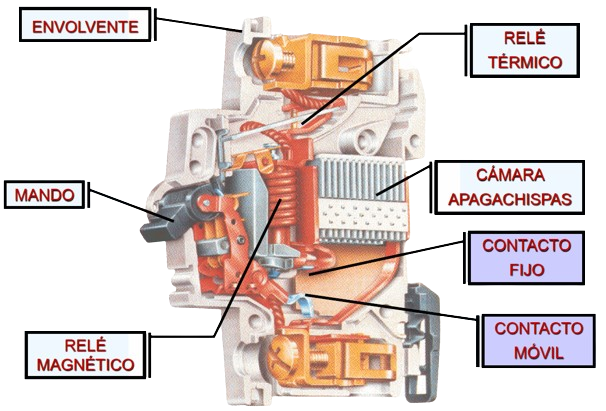
\includegraphics[width=0.7\linewidth]{Images/1}
	\label{fig:1}
\end{figure}

\subsection{Contacto}
Los elementos mecánicos que hacen contacto para que conduzca la corriente no son iguales que la superficie total de los contactos debido a las imperfecciones en el acabado superficial de estas. Por tanto, se habla de superficie aparente (la ideal) y real de contacto.
\newline

Se habla de conductores principales cuando han de soportar las intensidades de apertura y cierre. Para ello, han de tener las siguientes características:
\begin{itemize}
	\item Garantizar la conducción
	\item Tener una buena velocidad de desconexión
	\item Soportar esfuerzos térmicos y mecánicos del arco eléctrico
\end{itemize}

En cuanto a los materiales empleados para estos contactos, se emplea cobre hasta los 100 A y recubrimientos de aleaciones de plata que han de cumplir lo siguiente:
\begin{itemize}
	\item Baja resistividad eléctrica
	\item	Elevada temperatura de fusión
	\item Elevada resistencia a la corrosión
	\item Elevada resistencia a la oxidación
	\item Elevada resistencia a los agentes atmosféricos
	\item Elevada resistencia mecánica a la percusión
	\item Elevada resistencia mecánica al frotamiento
\end{itemize}
\subsection{Cámara de ruptura}
Tiene la función de absorber la energía de la tensión de arco, garantizar las condiciones suficientes de regeneración eléctrica y la evolución adecuada de la tensión de arco.
\subsection{Precámara}
Es el volumen de separación entre la zona de contactos y la cámara de ruptura. Se emplea para desplazar el arco al interior de la cámara y favorecer el alargamiento del arco. Para ello, se aprovecha la sobrepresión en la precámara de manera que la sección de la columna de arco se encuentra reducida y la diferencia de presión con la cámara de ruptura favorece la entrada y permanencia del arco en su interior.
\newline

Para ello, los fabricantes emplean distintas soluciones como la repulsión de contactos con pantallas magnéticas o el aprovechamiento de la fuerza de Lorentz creada por los campos magnéticos.
\subsubsection{Tobera}
Es el elemento constructivo que permite desplazar el arco y evitar su retroceso mediante su diseño. 
\begin{figure}[H]
	\centering
			\begin{adjustbox}{width=0.6\textwidth}
		\begin{circuitikz}
			\tikzstyle{every node}=[font=\normalsize]
			\draw [ color={rgb,255:red,0; green,30; blue,255}, short] (2.5,13.75) -- (2.5,10.25);
			\draw [short] (2.5,13.5) .. controls (8.25,11.75) and (7,12.75) .. (8.75,13.5);
			\draw [ color={rgb,255:red,0; green,30; blue,255}, short] (8.75,13.75) -- (8.75,10.25);
			\draw [short] (2.5,10.5) .. controls (8.25,12.25) and (7,11.25) .. (8.75,10.5);
			\draw [ color={rgb,255:red,0; green,30; blue,255}, short] (6.75,12.75) -- (6.75,11.25);
			\node [font=\normalsize, color={rgb,255:red,0; green,30; blue,255}] at (6.75,13) {$p_m$};
			\node [font=\normalsize, color={rgb,255:red,0; green,30; blue,255}] at (8.75,14) {$p_2$};
			\node [font=\normalsize, color={rgb,255:red,0; green,30; blue,255}] at (2.5,14) {$p_1$};
			\draw [dashed] (2.25,12) -- (9,12);
			\draw [ color={rgb,255:red,0; green,219; blue,73}, ->, >=Stealth] (2.75,12.5) -- (3.75,12.5);
			\draw [ color={rgb,255:red,0; green,219; blue,73}, ->, >=Stealth] (2.75,11.5) -- (3.75,11.5);
			\draw [ color={rgb,255:red,0; green,219; blue,73}, ->, >=Stealth] (8,12.5) -- (8.5,12.5);
			\draw [ color={rgb,255:red,0; green,219; blue,73}, ->, >=Stealth] (8,11.5) -- (8.5,11.5);
			\node [font=\normalsize, color={rgb,255:red,0; green,30; blue,255}] at (6.75,10.75) {Sección minima};
		\end{circuitikz}
			\end{adjustbox}
\end{figure}
\subsection{Cámara de ruptura}
Es el conjunto de separadores dispuestos transversalmente al arco eléctrico para fraccionarlo y absorber su calor. Por tanto, es el elemento principal para determinar si una protección puede abrir un cortocircuito, pues, existe un límite superior de intensidad por encima del cual el arco permanece entre los separadores.
\begin{figure}[H]
	\centering
	\begin{minipage}{0.4\textwidth}
		\begin{adjustbox}{width=0.9\textwidth}
			\centering
					\begin{circuitikz}
						\tikzstyle{every node}=[font=\normalsize]
						\draw  (3.25,14.25) rectangle (8.25,13.5);
						\draw  (3.25,9.25) rectangle (8.25,8.5);
						\draw [ color={rgb,255:red,51; green,0; blue,255} ] (3,9.75) rectangle (6,9.5);
						\draw [ color={rgb,255:red,51; green,0; blue,255} ] (3,10.25) rectangle (6,10);
						\draw [ color={rgb,255:red,51; green,0; blue,255} ] (3,10.75) rectangle (6,10.5);
						\draw [ color={rgb,255:red,51; green,0; blue,255} ] (3,11.25) rectangle (6,11);
						\draw [ color={rgb,255:red,51; green,0; blue,255} ] (3,11.75) rectangle (6,11.5);
						\draw [ color={rgb,255:red,51; green,0; blue,255} ] (3,12.25) rectangle (6,12);
						\draw [ color={rgb,255:red,51; green,0; blue,255} ] (3,12.75) rectangle (6,12.5);
						\draw [ color={rgb,255:red,51; green,0; blue,255} ] (3,13.25) rectangle (6,13);
						\draw [<->, >=Stealth] (2.25,13.5) -- (2.25,9.25);
						\draw [short] (2.25,9.25) -- (3.25,9.25);
						\draw [short] (2.25,13.5) -- (3.25,13.5);
						\node [font=\normalsize] at (1.75,11.5) {L};
						\draw [ color={rgb,255:red,56; green,6; blue,255}, <->, >=Stealth] (2.75,13.25) -- (2.75,9.5);
						\node [font=\normalsize, color={rgb,255:red,56; green,6; blue,255}] at (2.5,11.5) {N};
					\end{circuitikz}
		\end{adjustbox}
	\end{minipage}
	\begin{minipage}{0.4\textwidth}
		\centering
			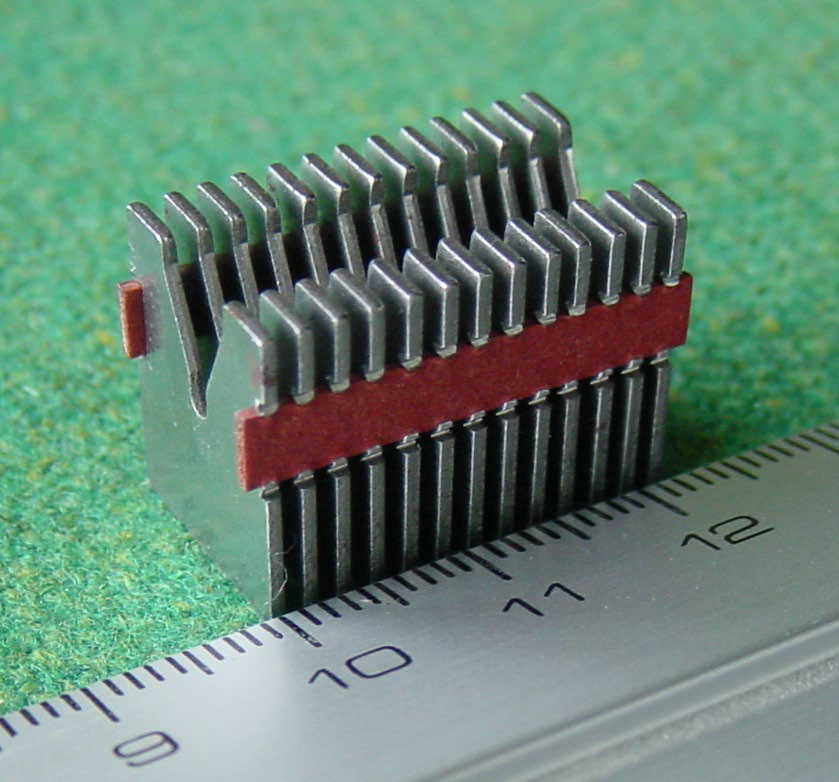
\includegraphics[width=0.7\linewidth]{Images/2}
	\end{minipage}
\end{figure}

La tensión de arco en estas condiciones quedaría como:
\begin{equation}
	U_a=N\cdot U_{AC}+\left(L-N\cdot e\right)U_L
\end{equation}

Donde $U_a$ es la tensión de arco, $U_{AC} $ la tensión anódica y catódica, $U_L$ la caída de tensión por unidad de longitud, $e$ el espesor de la placa separadora, $N$ el número de separadores y $L$ la longitud de la cámara de ruptura. 
\newline

A veces, se emplean cámaras de ruptura especiales como el bloque limitador. El bloque limitador mediante repulsión por conexiones cruzadas, repulsión en el contacto móvil y doble ruptura permite reducir la corriente limitada para que sea un orden de magnitud inferior a la corriente sin limitar, en una cámara de ruptura normal la reducción no es tan significativa.
\subsection{Relé}
Existen numerosos relés según el tipo de protección donde destacan el relé térmico y el relé magnético.
\newline

Según el principio de funcionamiento se distinguen varios tipos de relés:
\begin{itemize}
	\item Electromecánicos:
	\begin{itemize}
		\item Relé térmico: basado en un bimetal. Limita sobrecargas
		\item Relé magnético: basado en una bobina. Limita cortocircuitos
	\end{itemize}
	\item Electrónicos: tienen las siguientes ventajas
	\begin{itemize}
		\item Mayor capacidad de regulación y ajuste
		\item Funcionamiento independiente de la temperatura ambiente
		\item Facilidad de coordinación con otras protecciones
		\item Permite funciones adicionales
	\end{itemize}
\end{itemize}
\subsection{Relé térmico mecánico}
El bimetal consiste en la soldadura de dos láminas metálicas con diferente coeficiente de dilatación. Normalmente se usa cobre e Invar.
\begin{figure}[H]
	\centering
	\begin{minipage}{0.45\textwidth}
			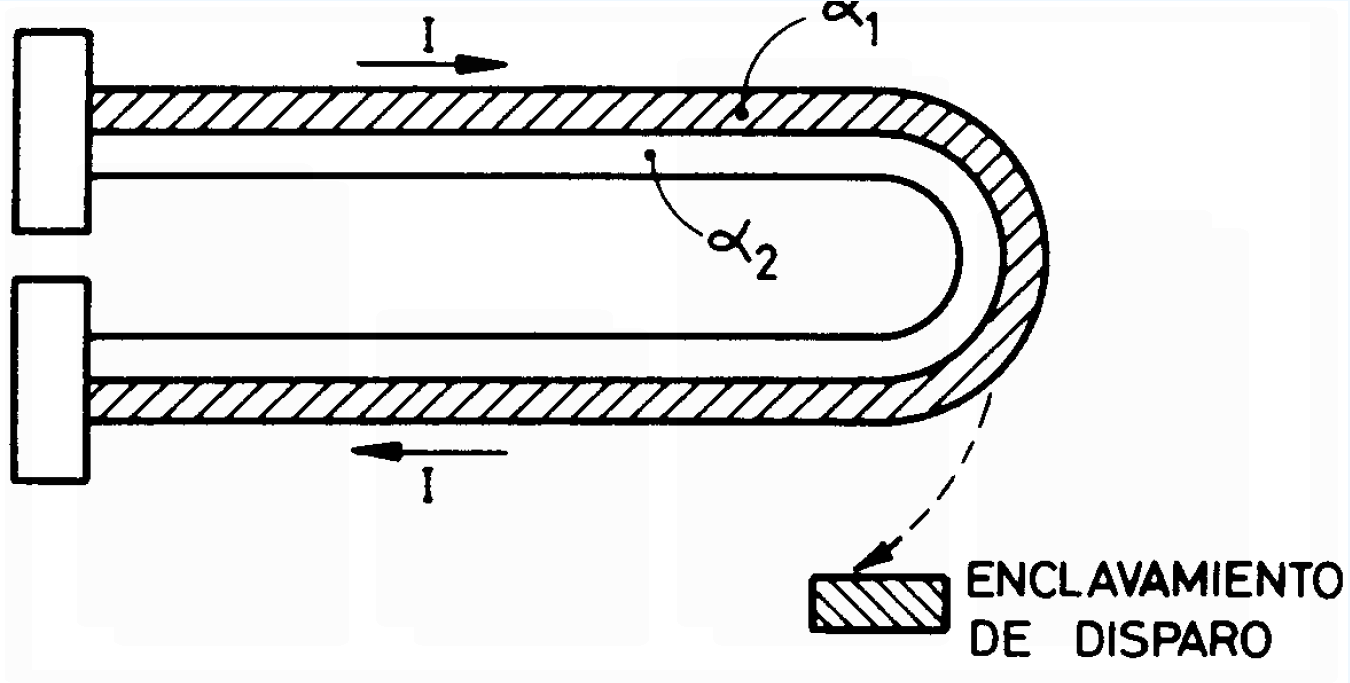
\includegraphics[width=0.7\linewidth]{Images/6}
			\caption{Calentamiento directo\newline (hasta 15 A)}
			\label{fig:6}
	\end{minipage}
	\begin{minipage}{0.45\textwidth}
		\centering
		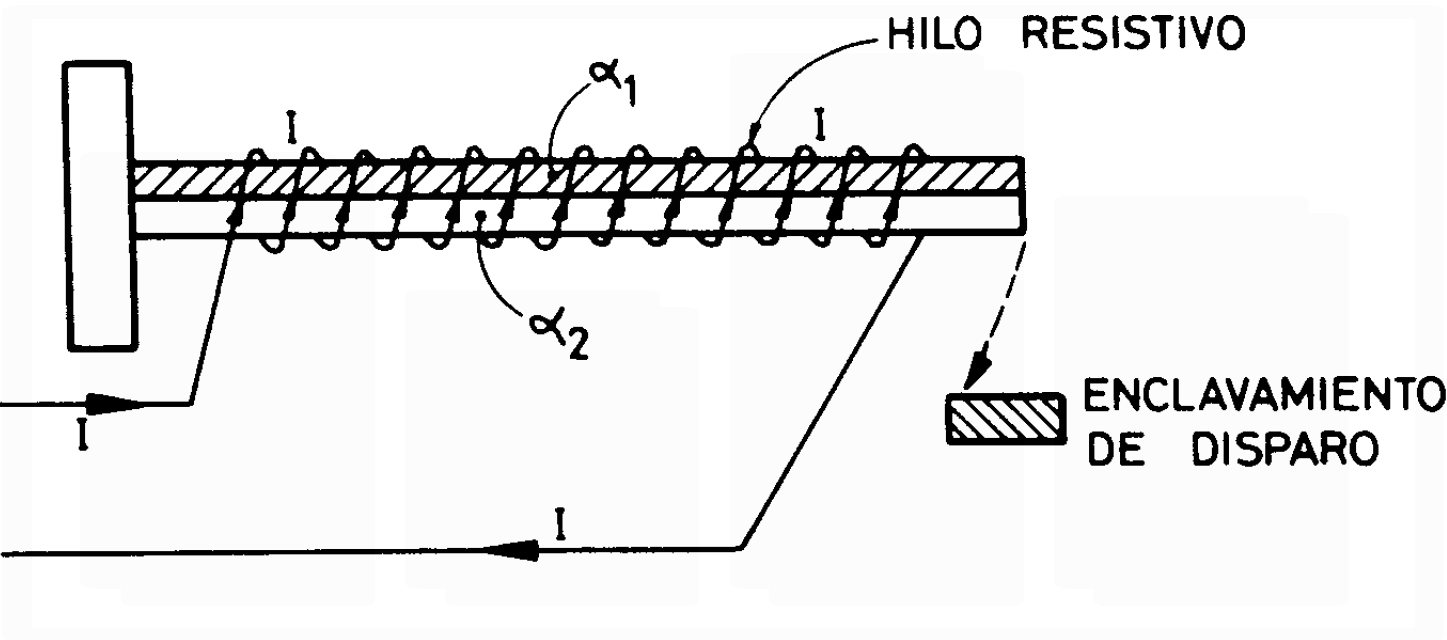
\includegraphics[width=0.7\linewidth]{Images/7}
		\caption{Calentamiento indirecto}
		\label{fig:7}
	\end{minipage}
\end{figure}

Para su disparo el relé se basa en la ley de Joule con flujo constante:
\begin{equation}
	I^2t=cte
\end{equation}

Su curva de disparo:
\begin{figure}[H]
	\centering
	\begin{minipage}{0.6\textwidth}
		\centering
		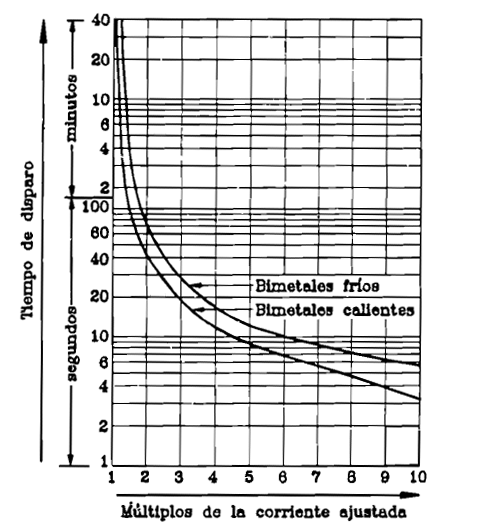
\includegraphics[width=0.7\linewidth]{Images/8}
	\end{minipage}
	\begin{minipage}{0.35\textwidth}
		El comportamiento del bimetal depende de la intensidad, el tiempo, la temperatura inicial, la temperatura ambiente y la frecuencia de la señal.
	\end{minipage}
\end{figure}	
\subsection{Relé instantáneo magnético}
Se habla de un relé con disparo prácticamente instantáneo. No es instantáneo debido a la inercia mecánica y magnética del sistema.
\newline

Su curva de disparo:
\begin{figure}[H]
	\centering
	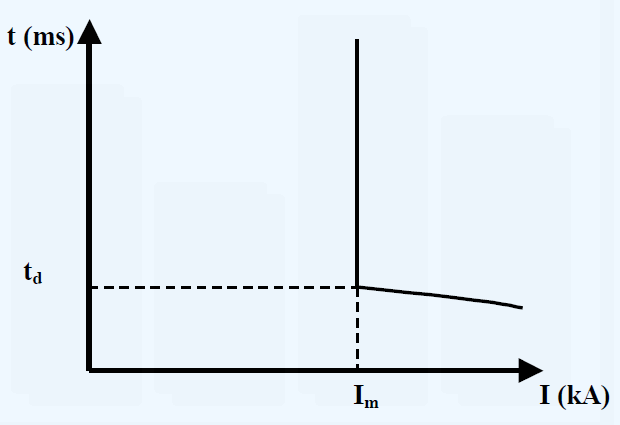
\includegraphics[width=0.5\linewidth]{Images/9}
	\label{fig:9}
\end{figure}

\subsection{Curvas de actuación de un relé de sobreintensidad electrónico}
\begin{figure}[H]
	\centering
	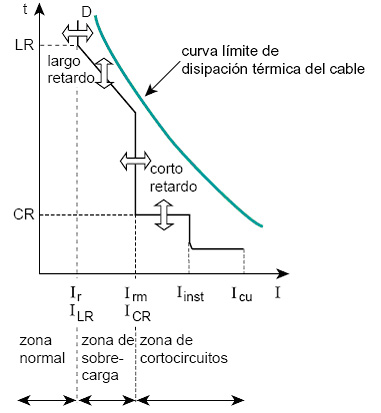
\includegraphics[width=0.5\linewidth]{Images/10}
	\label{fig:10}
\end{figure}

\section{Tipos constructivos de interruptores}
\subsection{Pequeños interruptores automáticos}
\begin{figure}[H]
	\centering
	
	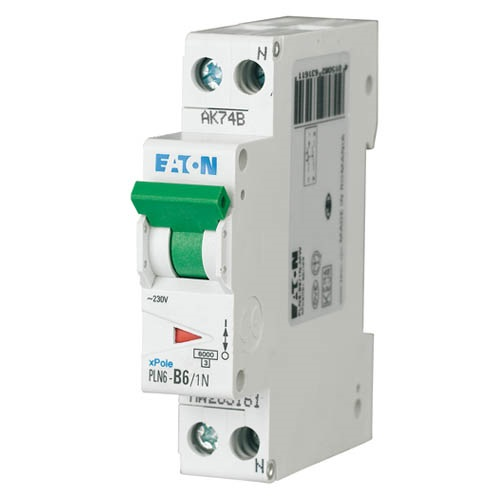
\includegraphics[width=0.3\linewidth]{Images/3}
	\label{fig:3}
\end{figure}

\subsection{Caja moldeada}
\begin{figure}[H]
	\centering
	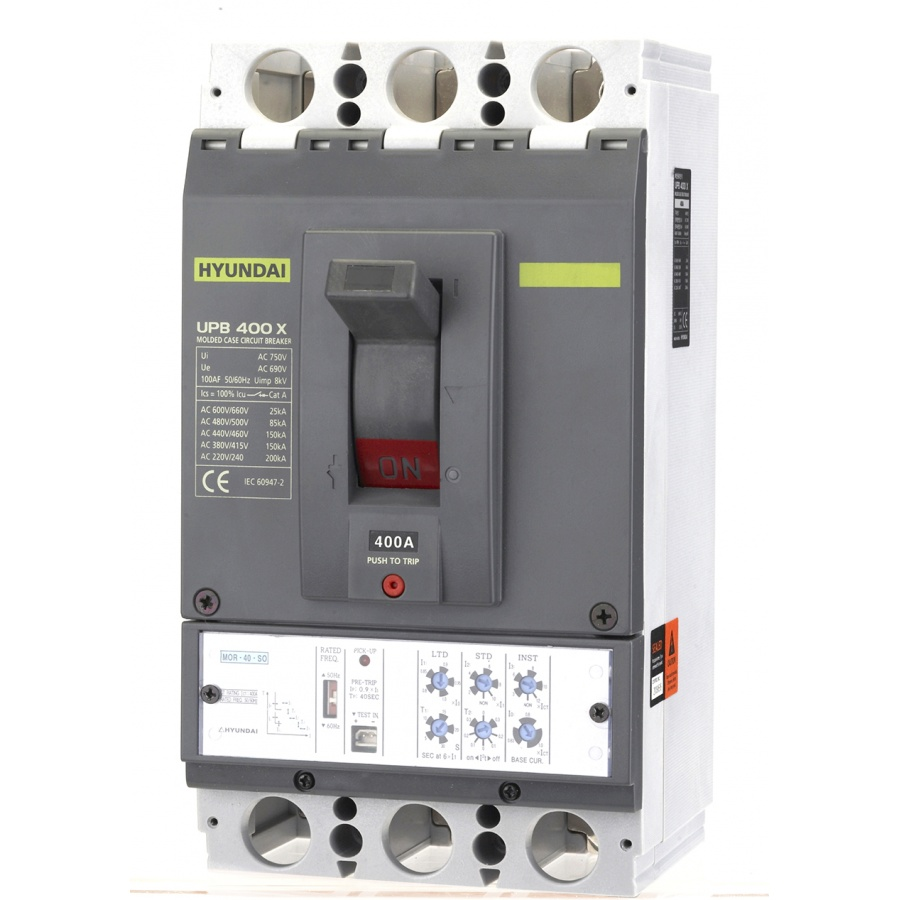
\includegraphics[width=0.3\linewidth]{Images/4}
	\label{fig:4}
\end{figure}

\subsection{Bastidor abierto}
\begin{figure}[H]
	\centering
	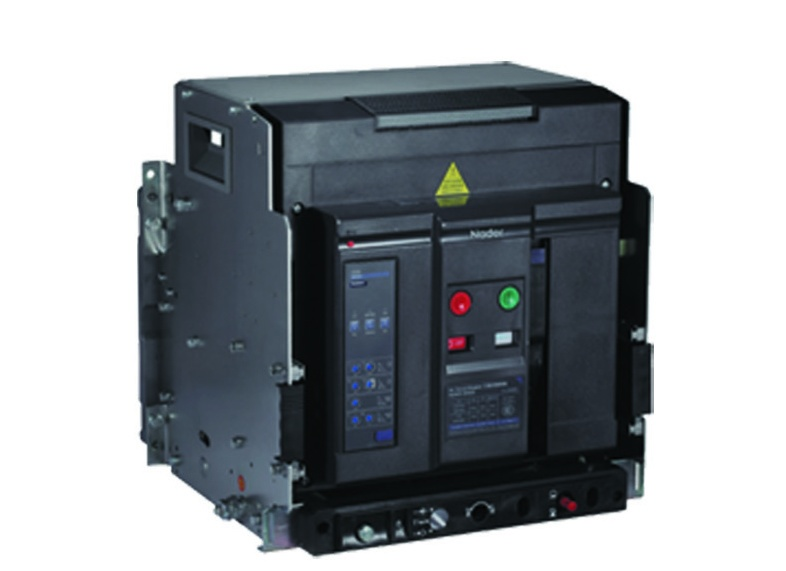
\includegraphics[width=0.3\linewidth]{Images/5}
	\label{fig:5}
\end{figure}

\section{Normativa}
La normativa de domésticos (60898) es más restrictiva que la de industriales (60947) y los pequeños interruptores automáticos pueden ensayarse con cualquiera de ellas según su aplicación.
\subsection{UNE ENE 60898-1}
Accesorios eléctricos. Interruptores automáticos para instalaciones domésticas y análogas para la protección contra sobreintensidades. Parte 1: Interruptores automáticos para funcionamiento en corriente alterna.
\subsection{UNE EN 60947-2}
Aparamentade baja tensión. Parte 2: Interruptores automáticos.
\section{Mandos}
Según el accionamiento se habla de:
\begin{itemize}
	\item Maneta: existe un elemento parecido a un mango que permite manipular la protección (sobresale)
	\item Maneta rotativa: como la maneta pero de rotación
	\item Rotativo: vienen con una rueda que no sobresale (no hay hueco entre mando y automático)
	\item Palanca o manivela: existe un elemento que sobresale del automático (más que la maneta)
	\item Pulsadores
\end{itemize}
\section{Envolvente}
Es el bloque donde se montan los componentes del interruptor automático. Normalmente esta compuesto de plásticos termoendurecidos prensados o metales. Esta envolvente debe garantizar el aislamiento entre polos, tener las características mecánicas necesarias y carecer de higroscopicidad (capacidad de absorber humedad).
\section{Elementos de seguridad}
En función de la seguridad que da el interruptor para manipular la red y asegurarte de que la red no se reconecte se distingue:
\begin{itemize}
	\item Seguridad de puerta: permite una fijación en la puerta al girar un elemento interior
	\item De candado: permite colocar un candado para enclavarse en la posición de apagado
	\item De llave: vienen con una llave que impide manipularlo sin ella
\end{itemize}
\section{Interruptores automáticos inteligentes}
Suelen denominarse como Smart MCB. Permiten registrar su estado, variables físicas y comunicación con dispositivos externos.
\section{Comparativa fusible contra interruptor automático}
Inconvenientes de los fusibles:
\begin{itemize}
	\item Necesidad de disponer de repuestos
	\item Posibilidad de colocar fusibles de calibre no adecuado
	\item Funcionamiento por debajo del valor nominal
\end{itemize}

Ventajas de los interruptores automáticos:
\begin{itemize}
	\item Recuperación automática
	\item Mecanismo de disparo independiente del mando
	\item Mayor seguridad frente a contactos directos
	\item Desconexión de todos los polos
	\item Permite maniobras de servicio moderadas > 10.000
	\item Curva constante: no envejecimiento (adecuado tarificación)
	\item Comprobación de características sin destrucción
	\item Posibilidad de funciones adicionales
\end{itemize}